% Pour toute question sur l'utilisation de cette classe, écrivez à jerome.soucy(at)ulaval.ca
% Nécessite la classe Evaluation.sty dans le même dossier ou dans le PATH de votre système
% Nécessite le fichier logo_ul.pdf dans le même dossier un dans le PATH de votre système
\def\Ponderation{35}
\def\SigleNumero{STT-1000}
\def\NomCours{Probabilités et statistique}
\def\DateEvaluation{27 octobre 2022 de 18h30 à 21h20}
\def\Session{Été 2021}
\def\NomEvaluation{Examen 1}

% Ne rien mettre entre les accolades si l'enseignant (ou l'enseignante) est aussi le coordonnateur (ou la coordonnatrice)
\def\Coordonnatrice{}
\def\Coordonnateur{}

% Ne rien mettre entre les accolades s'il y a plus d'une section
\def\Enseignant{}
\def\Enseignante{}

% Ne rien mettre entre les accolades s'il s'agit d'un cours à section unique
% Mettre le nom de chacun des enseignants et enseignantes entre les accolades
% Une case à cocher sera générée pour chacune des sections
\def\SectionA{Anne-Sophie Charest}
\def\SectionB{Julien Miron}
\def\SectionC{}
\def\SectionD{}

% Concerne seulement les travaux pratiques : écrire entre les accolades le nombre maximal de membres pour une équipe
\def\NombreLignes{}		

% Si vous souhaitez qu'apparaisse une déclaration d'honneur au bas de la première page, écrivez quelque chose entre les accolades
\def\EnLigne{}

\def\Directives{
\begin{enumerate}
\item Matériel autorisé:
\begin{itemize}
\item Calculatrice scientifique {\bf autorisée par la faculté des sciences et de génie};
\item Le feuillet de formules fourni avec l'examen. Celui-ci inclut la table de la loi normale.
\end{itemize}
\item Assurez-vous que cette \'evaluation comporte \numquestions ~questions réparties sur \numpages{}~pages, pour un total de \numpoints{}~points.\
\item \textbf{Veuillez ne pas débrocher votre examen.}
\item Veuillez déposer votre carte d'identité \textbf{admise} avec photo sur votre bureau.\
\item Vous devez\textbf{ justifier votre réponse} par une démarche claire, sauf pour les questions à choix de réponse.\
\item Pour les questions à choix de réponse, vous pouvez mettre un X, un crochet ($\checkmark$) ou remplir la case.
\item Le verso des feuilles peut être utilisé comme brouillon, \textbf{mais ne sera pas corrigé}. Attention à ne rien débrocher.
\end{enumerate}
}

% Veuillez indiquer le type d'évaluation entre crochets
% Examen : option à choisir pour un examen présentiel qui sera corrigé de manière classique. Un tableau des points sera affiché sur la page couverture.
% Gradescope : option à choisir pour un examen qui sera corrigé via Gradescope. Aucun tableau de pointage n'apparaîtra et il y a quelques différences au niveau de la mise en page
% TPS :
% TPF :
% Devoir :
\documentclass[Gradescope]{Evaluation}
\usepackage{multicol,graphicx}
\begin{document}

\newpage
%%%%%%%%%%%%%%%% QUESTION %%%%%%%%%%%%%%%%
\begin{questions}
\question[3] Considérons le montage électronique représenté ci-dessous. %module 1
	
	\begin{figure}[h!]
		\label{fig:montage}
		\begin{center}	\begin{tikzpicture}	
			% bandes verticales
			\draw (0,0)--(1,0);
			\draw (1,0)--(1,1);
			\draw (1,0)--(1,-1);
			\draw (1,1)--(1.7,1);
			\draw (2.3,1)--(3,1);
			\draw (1,-1)--(1.7,-1);
			\draw (2.3,-1)--(3,-1);
			\node at (2,1) {A1};
			\node at (2,-1) {A2};
			\draw (3,-1)--(3,1);
			\draw (3,0)--(4,0);
			\node at (2,-1.6) {Bloc A};
			\end{tikzpicture} \end{center}
		\vspace{-0.8cm}\end{figure}
	Le bloc A contient deux éléments. Nous avons que
	\begin{itemize}
		\item L'élément A1 fonctionne avec une probabilité de 0,70.
		\item L'élément A2 fonctionne avec une probabilité de 0,70.
	\end{itemize}
	Pour que le montage fonctionne, au moins un élément du bloc A doit fonctionner. Les éléments d'un bloc fonctionnent de façon indépendante.
	
	\vspace{0,3cm}
	


Quelle est la probabilité que le montage ne fonctionne pas? 

\begin{oneparcheckboxes}
\choice $0,49$
\choice $0,70$
\choice $0,03$
\choice $0,91$
\CorrectChoice $0,09$
\end{oneparcheckboxes}

\vspace{1cm}

\begin{solution}
$P(\bar{F})= P(\bar{A1}) \times P(\bar{A2}) = 1 - \left[\left\{1-P\left(\bar{A_1}\right)\right\}\left\{1-P\left(\bar{A_2}\right)\right\}\right]=1-0,3^2=0,91$
\end{solution}

\question[3] Soit $A$ et $B$, deux événements de $S$. Nous savons que $$0<P(A)+P(B)<1.$$ Laquelle des affirmations suivantes est tout le temps vraie?
%modules 1 et 2

\begin{checkboxes}
    \choice $A$ et $B$ sont indépendants
    \choice $A$ et $B$ forment une partition de l'espace échantillonnal
    \correctchoice $P(A \cup B) > 0$
    \choice $P(A \cap B) > 0$
    \choice $A$ et $B$ sont mutuellement exclusifs
\end{checkboxes}

\begin{solution}
Comme $P(A)+P(B)>0$, on a que $P(A)>0$ ou $P(B)>0$.\\ 
$A \perp B$ si $P(A\cap B)=P(A)P(B)$. Nous n'avons pas suffisamment d'informations.\\
Comme $P(A)+P(B)<1$, ils ne forment pas une partition de l'espace échantillonnal.\\
Suite\\
Réponse C)
\end{solution}

\vspace{1cm}



\question[3] Laquelle des fonctions suivantes est une fonction de masse de probabilité? %module 3

\begin{checkboxes}
\choice $P_X(a)=\left\{
\begin{array}{ll}
a  & \mbox{ si } a>0, \\
0 & \mbox{sinon}
\end{array}
\right.$

\vspace{0.3cm}

\choice $ \displaystyle P_X(b)= \left\{
\begin{array}{ll}
0,5 &\mbox{ si } b \in \{0,1,2\}, \\
0 & \mbox{sinon}
\end{array}
\right.$

\vspace{0.3cm}

\CorrectChoice $ \displaystyle P_X(c)= \left\{
\begin{array}{ll}
0,5  & \mbox{ si } c=-2, \\
0,25 & \mbox{ si } c \in \{1, 2\} \\
0 & \mbox{sinon}
\end{array}
\right. $

\vspace{0.3cm}

\choice $P_X(d)=\left\{
\begin{array}{ll}
d  & \mbox{ si } d\in \{1,2,3,4,5,6\}, \\
0 & \mbox{sinon}
\end{array}
\right.$
\end{checkboxes}

\vspace{1cm}

\begin{solution}
A) a est continue et quand a>1, P(a)>1. B) a une somme de P(b) > 1. D) a des probabilités >1. C) est la bonne réponse.
\end{solution}

\question[3] Soit $A\subset B \subset S$ où $S$ est l'ensemble universel.\\
Laquelle des expressions suivantes est toujours vraie si $P(A)~>~0$~et~$P(B)~>~0$?

\begin{oneparcheckboxes}
    \choice $P(A) > P(B)$
    \choice $P(A)+P(B)<1$
    \correctchoice $P(A|B)\geq P(A)$
    \choice $P(B|A)=0$
\end{oneparcheckboxes}

\vspace{1cm}

\question[3] Si $X$ est une variable aléatoire normale de moyenne $\mu$ et de variance $\sigma^2$, nous pouvons écrire $X\sim\mathcal{N}(\mu, \sigma^2)$. Laquelle des affirmations suivantes est vraie? %module 5

\begin{checkboxes}
\choice $\displaystyle Z=\frac{X-\mu}{\sigma^2}\sim \mathcal{N}(0, 1)$
\choice $\displaystyle Y=3X+2 \sim \mathcal{N}(3\mu+2, 9\sigma^2 + 4)$
\CorrectChoice La fonction de densité de $X$ est symétrique
\choice La fonction de répartition de $X$ est symétrique
\end{checkboxes}

\vspace{1cm}

\question[5]
Une population est formée à 40\% d'enfants et à 60\% d'adultes. On sait que parmi les enfants 95\% aiment le chocolat, et que parmi les adultes seulement 70\% aiment le chocolat. On choisit par hasard une personne parmi celles qui aiment le chocolat. Quelle est la probabilité que celle-ci soit un enfant? Justifiez vos calculs.
\begin{solution}
Soit la notation suivante : 
E : être un enfant
A: être un adulte
C: aimer le chocolat
On sait que $P(E)=0.4$, $P(A)=0.6$, $P(C|E)=0.95$ et $P(C|A)=0.7$.
On cherche $P(E|C)$.
On doit ici utiliser le théorème de Bayes. On a donc 
\begin{align}
    P(E|C) &= \frac{P(C|E)P(E)}{P(C)}\\
    &= \frac{P(C|E)P(E)}{P(C|E)P(E) + P(C|A)P(A)} \\
    &= \frac{0.95 * 0.4}{0.95 * 0.4 + 0.7*0.6}\\
    &= \frac{0.38}{0.38+0.42} \\
    &= 0.457
\end{align}
\end{solution}

\vspace{5cm}



\vspace{8cm}


\newpage

\question Un producteur de Vacherin Fribourgeois sait que le poids d'une de ses meules de fromage, $X$, est une variable aléatoire de loi normale $\mu=15$ kg et $\sigma^2 = 4$ kg$^2$.%module 5

\begin{parts}
    \part[6] Quelle est le poids $p$, tel que $P(X>p)=0,15866$? Laissez des traces de votre démarche.
    \begin{solution}
        On cherche $P(X>p)=0,15866$ sachant que $X\sim\mathcal{N}(15, 4)$
        \begin{align*}
            P(X>p)&= P\left(\frac{X-15}{2}>\frac{p-15}{2}\right)\\
            0,15866&= P\left(Z>\frac{p-15}{2}\right) \ \ \text{ où } Z\sim \mathcal{N}(0,1)\\
            1-0,15866 &= P\left(Z\leq\frac{p-15}{2}\right)\\
           1-0,15866 &= \Phi\left(\frac{p-15}{2}\right)\\
           0,84134 &= \Phi\left(\frac{p-15}{2}\right)\\
           \Phi^{-1}(0,84134) &= \frac{p-15}{2}\\
           1&= \frac{p-15}{2}\\
           p &= 17
        \end{align*}
    \end{solution}
    \vspace{8cm}
    \part[8] Le producteur doit envoyer 100 meules à un supermarché. Une compagnie de transport lui charge 1500\$ si le poids des 100 meules est inférieur à 1800 kg ou 2000\$ si le poids est supérieur ou égal à 1800~kg. Quelle est l'espérance du prix que le producteur devra payer pour le transport avec cette compagnie? Laissez des traces de votre démarche.

    \begin{solution}
     Soit $Y=X_1+...+X_100$, $Y\sim\mathcal{N}(100*15; 100*4)$, $Y\sim\mathcal{N}(1500, 400)$.
     
     On commence par trouver la probabilité que $Y>1800$. 
     \begin{align*}
         P(Y>1800)&= P(Z>\frac{1800-1500}{20})\\
         &= P(Z>15)\\
         &\approx 0
     \end{align*}
     
     Soit $W$ la variable qui décrit si le poids est supérieur à 1800kg, $W\sim$Bernoulli$(\approx 0)$. On sait que $E(W)\approx0$.
     
     Soit $T$ qui décrit le prix que payera le producteur, $T=1500+500W$. D'où $E(T)=1500+500E(W)\approx 1500$

     OU

     $E(T)\approx1500 * 1+2000 * 0$. Il s'agit de la somme sur les possibilité de $T$ multiplié par la probabilité (l'espérance...).
    \end{solution}
    
\end{parts}
\newpage
\question Le nombre de tentatives d'infiltration dans un serveur sécurisé se fait selon un processus de Poisson. Le temps moyen entre deux tentatives est $12$ minutes. %modules 4 et 5
\begin{parts}
    \part[5] Quelle est la probabilité que le temps entre deux tentatives soit supérieur à $20$ minutes. Laissez des traces de votre démarche.
\begin{solution}
    Si le temps moyen $X$ entre deux tentatives est de 12 minutes, $X\sim \exp(\lambda = 1/12)$. D'où 

    \begin{align*}
        P(X>20)&=\int _{20}^\infty \frac{1}{12}\exp\left(\frac{-x}{12}\right)dx\\
        &= \left.-\exp\left(\frac{-x}{12}\right)\right|_{20}^\infty\\
        &= \exp\left(-20/12\right)\\
        &\approx 0,189.
    \end{align*}

    OU DIRECTEMENT

        \begin{align*}
        P(X>20)&=1-[1-\exp\left(-20/12\right)] \text{ par la fonction de répartition }\\
        &\approx 0,189.
    \end{align*}


    OU 

    Si le temps moyen entre deux tentatives est de 12 minutes, il s'agit d'un processus de Poisson d'intensité 1 tentative / 12 minutes. Sur 20 minutes, le \# de tentatives $Y$ suit donc une Poisson($\mu = 5/3$). On cherche donc $P(Y=0)$.

    \begin{align*}
        P(Y=0) &= \frac{\exp(-5/3)\left(\frac{-5}{3}\right)^0}{0!}\\
        &= \exp(-5/3)\\
        &\approx 0,189
    \end{align*}
    
\end{solution}
%Il faut intégrer l'exponentielle ici. 
    \vspace{4cm}

%    \part[3] Si on voulait exprimer ce processus en heure, quelle serait le nouveau paramètre d'intensité? On veut que l'unité de temps soit $1$ heure.

    \vspace{2cm}

    \part[5] Une équipe d'experts tente de répliquer les tentatives d'infiltration dans le but d'améliorer les défenses du serveur. Ils lancent une séquence de tentatives d'infiltration selon le même processus de Poisson. Quelle est l'espérance du temps total pour lancer les 8 tentatives d'infiltration? Justifiez votre réponse.
    \begin{solution}
        Si $W$ est le temps pour lancer 8 tentatives, $W\sim \text{Gamma}(8; 1/12)$, donc $E(W)=\frac{8}{1/12}=96$ minutes.
    \end{solution}
\end{parts}
\newpage


\question On lance un dé \textit{non équilibré} dont le résultat est la variable aléatoire $X$ et a la fonction de masse suivante: %modules 3 (12 pts) et 4 (3 pts)

\begin{center}
    $P_X(x)=\left\{
			\displaystyle \begin{array}{ll}
			\displaystyle \frac{x}{21}  & \mbox{ si } x\in{1,2,3,4,5,6}, \\
			0 & \mbox{sinon}.
			\end{array}
			\right.$
\end{center}

\begin{parts}
%\part[3] Montrez que $P_X(x)$ est bien une fonction de masse.
%\vspace{3cm}

\part[2] Quelle est la probabilité que le résultat d'un lancer soit un nombre pair?
\vspace{3cm}

\part[5] Quelle est l'espérance de la variable aléatoire $X$? Laissez des traces de votre démarche.


\vspace{6.5cm}

\part[3] On lance le dé 10 fois. Soit $Y$ la variable aléatoire qui compte le nombre total de «$6$» obtenus. Quelle est la distribution de $Y$? Il faut le nom et tous les paramètres.
 
\end{parts}



\newpage
\question Après un certain nombre de tours pendant une partie de \textit{Scrabble}, les 15 lettres suivantes n'ont toujours pas été choisies et sont donc encore dans le sac:
$$\{a, e, i, g, h, l, n, o, p, t, t, v, v, w, x\}.$$

\begin{parts}
    \part[4] Si Alex doit piger 4 lettres au hasard dans le sac, quelle est la probabilité que ces lettres soit les lettres de son prénom, dans le bon ordre? Laissez des traces de votre démarche.
\begin{solution}
    Soit l'événement $A:$ Alex pige les lettres de son nom dans l'ordre.
    
    Comme l'ordre est important, la probabilité est

    \begin{align*}
        P(A)&=\frac{1}{15}\times\frac{1}{14}\times\frac{1}{13}\times\frac{1}{12}\\
        P(A)&= \frac{1}{32760}
    \end{align*}
\end{solution}

    \vspace{8cm} 
    \part[6] Supposons qu'Alex a pigé $\{i, g, t, w\}$. Il reste donc 
$\{a, e, h, l, n, o, p, t, v, v, x\}$ dans le sac. C'est maintenant au tour d'Eva de piger 4 lettres. Quelle est la probabilité que parmi ses 4 lettres, elle pige les lettres qui forment son prénom (peu importe l'ordre)? Laissez des traces de votre démarche.
\begin{solution}
     Soit l'événement $E:$ Eva pige au moins les 3 lettres de son nom peu importe l'ordre.
    
    Comme l'ordre n'est pas important.

    \begin{align*}
        P(E)&= \frac{\binom{1}{1}\binom{1}{1}\binom{2}{1}\binom{8}{1}}{\binom{11}{4}}\\
        &= \frac{16}{330}\\
        &\approx 0,0485
    \end{align*}
\end{solution}
\end{parts}
\newpage

\question Soit la variable aléatoire $X$ et sa fonction de répartition:  %module 3
$$F_X(x) = \left\{
			\begin{array}{ll}
			0  & \mbox{ si } x<0, \\
			\sqrt{x} & \mbox{ si } 0\leq x < 1\\
			1 & \mbox{ si } 1 \leq x.
			\end{array}
			\right. $$
\begin{parts}
    \part[5] En vous servant de la fonction de répartition, calculez $\displaystyle P(\left. 0,25\leq X \leq 0,81 \right| X > 0,16)$. Laissez des traces de votre démarche.

    \begin{solution}
        \begin{align*}
            P(\left. 0,25\leq X \leq 0,81 \right| X > 0,16) &= \frac{P( 0,25\leq X \leq 0,81 \cap X > 0,16)}{P(X > 0,16)}\\
            &= \frac{P( 0,25\leq X \leq 0,81  )}{P(X > 0,16)}\\
            &= \frac{F_X(0,81)-F_X(0,25)}{1-F_X(0,16)}\\
            &= \frac{\sqrt{0,81}-\sqrt{0,25}}{1-\sqrt{0,16}}\\
            &= \frac{0,9-0,5}{0,6}\\
            &= 2/3 \approx 0,67
        \end{align*}
    \end{solution}
    \vspace{8cm}
    
    \part[5] Quelle est la fonction de densité $f_X(x)$ de la variable aléatoire $X$? Laissez des traces de votre démarche.

    \begin{solution}
        On sait que $\displaystyle f_X(x)= \frac{d F_X(x)}{dx}$. Donc

        \begin{align*}
            \frac{d F_X(x)}{dx}&= \frac{d x^{1/2}}{dx} \text{ pour }0\leq x\leq 1\\
            &= \frac{x^{-1/2}}{2}
        \end{align*}
        On a donc 

        $$ f_X(x) = \left\{
			\begin{array}{ll}
			\displaystyle \frac{1}{2\sqrt{x}} & \mbox{ si } 0\leq x < 1\\
			0 & \mbox{ sinon }.
			\end{array}
			\right. $$
    \end{solution}
\end{parts}


\newpage


\newpage

\question On considère deux variables aléatoires discrètes $X_1$ et $X_2$ pour lesquelles la fonction de probabilité de masse conjointe est donnée par 

\begin{center}
\begin{tabular}{|cc||c|c|c|}\hline
$p(x_1,x_2)$ & & \multicolumn{3}{c|}{$x_2$}  \\ \cline{3-5}
 & & 0 & 2 & 4  \\ \hline
 & 0 & 0 & 3/15 & 3/15  \\ \hline
$x_1$ & 1 & 2/15 & 6/15  & 0  \\ \hline
 & 2 & 0 &  1/15  &  0 \\ \hline
\end{tabular}
\end{center}


\begin{parts}
\part[4] Donnez la distribution conditionnelle de $X_2$ sachant que $X_1 = 1$. Justifiez vos calculs.

\begin{solution}
 Par définition de la probabilité conditionnelle, on a 
$$P(X_2 = x | X_1 = 1) = \frac{P(X_2=x \cap X_1=1)}{P(X_1=1)}$$

On calcule d'abord $$P(X_1=1) = P(X_1=1 \cap X_2 = 0) + P(X_1=1 \cap X_2 = 2) + P(X_1=1 \cap X_2 = 4)  = 2/16 + 6/15 + 0 = 8/15.$$

On a donc 
$$P(X_2 = 0 | X_1 = 1) = \frac{P(X_2=0 \cap X_1=1)}{P(X_1=1)} = \frac{2/15}{8/15} = 1/4$$

On obtient de la même façon $P(X_2 = 2 | X_1 = 1) = \frac{6/15}{8/15} = 3/4$ et $P(X_2 = 2 | X_1 = 1) = \frac{0}{8/15} = 0.$
   
\end{solution}


\vspace{5cm}

\part[4] Sachant que $E(X_1) = 2/3$ et que $E(X_2) = 2$, calculez la covariance entre $X_1$ et $X_2$. Laissez des traces de votre démarche.

\begin{solution}
Il n'y a que deux combinaisons des variables $X_1$ et $X_2$ qui donnent un produit non-nul. On a donc
$$E(X_1X_2) = 2*6/15 + 4*1/15 = 16/15$$
La covariance est donc $E(X_1X_2)-E(X_1)E(X_2) = 16/15 - 2/3*2 = 16/15-4/3 = -4/15.$
\end{solution}

\vspace{6cm}

\part[4] Montrez, sans utiliser le résultat obtenu en (b), que les variables aléatoires $X_1$ et $X_2$ ne sont pas indépendantes?

\begin{solution}
On a calculé en (a) que $P(X_1=1) = 8/15$. 
On voit aussi que $P(X_2=4) = 3/15. $
Si Les variables aléatoires étaient indépendantes, alors on aurait $P(X_1=1 \cap X_2 = 4) = P(X_1=1)P(X_2=4) = 8/15 * 3/15 = 24/225.$ Or cette probabilité conjointe vaut plutôt zéro, montrant que les variables aléatoires ne sont pas indépendantes. 

(Plusieurs autres réponses possibles.)
\end{solution}

\end{parts}

\newpage 

\question[4]
Tracez un diagramme en boîte possible pour une distribution asymétrique à gauche, avec une médiane de 100, un écart interquartile de 20 et une seule donnée
extrême. Le graphique n'a pas à être exactement à l'échelle, mais prenez soin d'inclure
un axe gradué.

Plusieurs solutions possibles. S'assurer que la donnée extrême est à plus de 30 de la fin de la boite. 

\vspace{8cm}

\question Clara a un verger dans la municipalité de Saint-Coeur-de-Pomme et offre l'autocueillette de pommes. Elle veut savoir si les habitants de la municipalité de Saint-Coeur-de-Pomme aiment la sorte de pomme Vista Bella, qu'elle souhaite introduire dans son verger. Elle décide donc de faire un sondage. Elle choisit par échantillonnage aléatoire simple 100 personnes parmi les clients de son verger durant la fin de semaine du 8 au 10 octobre. Elle leur demande à tous s'ils aiment le goût de la pomme Vista Bella et note leurs réponses. \\

\begin{parts}
\part[3] Est-ce qu'il y a une erreur de couverture ici? Justifiez votre réponse. 

\begin{solution}
Oui. Il y a sous-couverture car certains habitants ne seront pas à son verger du 8 au 10 octobre. Il y a aussi sur-couverture car certains clients durant la fin de semaine ne seront pas des habitants de la municipalité. 
\end{solution}

\vspace{4cm}

\part[3]Expliquez ce que serait une erreur de mesure dans cet exemple.

\begin{solution}
Ce pourrait être une personne qui dit qu'elle aime la pomme Vista Bella, mais qui n'y a jamais goûté et qui en fait ne l'aime pas. 
\end{solution}

\vspace{4cm}

\newpage
\part[4] Clara veut aussi savoir si ses clients mettent en moyenne 50 livres de pommes dans ses paniers de 50 livres. Pour cela, elle pèse un échantillon de 15 paniers de 50 livres de pommes remplis par ses clients. Les données obtenues sont présentées dans le graphique ci-dessous.  

\begin{center}
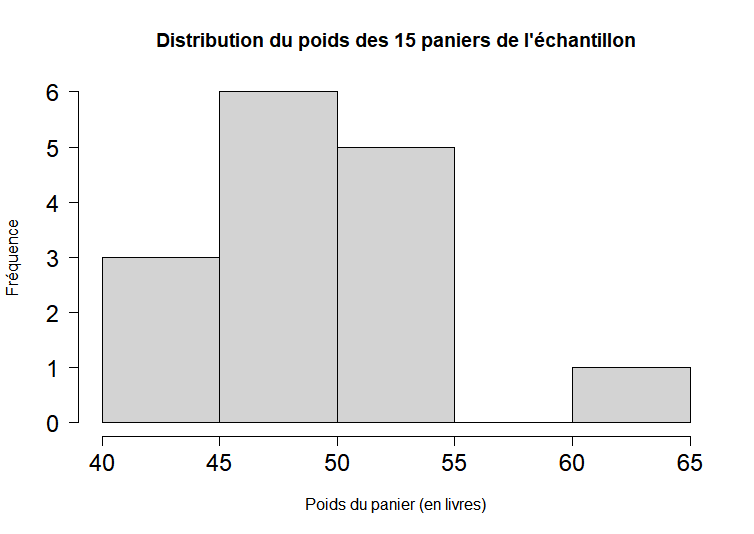
\includegraphics[scale=0.5]{HistPommes.png}
\end{center}

Utilisez le graphique ci-dessus pour estimer le poids moyen des 15 paniers de son échantillon. Laissez des traces de votre démarche.

\vspace{5cm}

\begin{solution}
On calcule $(1/15) * ( 42,5 *3 + 47,5*6 + 52,5 *5 + 57,5*0 + 62,5*1) = 737.5/15 = 49,1666$
\end{solution}

%\part[4]
%Supposons qu'on veuille faire un nouvel histogramme avec seulement trois rectangles : un premier pour les paniers de 40 à 50 livres, un deuxième pour les paniers de 50 à 55 livres et un troisième pour les paniers de 55 à 65 livres. Si la hauteur du premier rectangle est de 10 cm, quelle sera la hauteur du deuxième rectangle? 

\end{parts}




\end{questions}
\end{document} 
